\chapter{Analysis }

The following section will give an analytic insight to the steps required for designing the proposed software in relation to a business use case, Identify some of the problems that may arise and outline objectives for implementation.

An article by \citeauthor{hague} for the B2B international states that understanding a customers satisifaction rate is important as it can show where is the business is doing well or where it needs improvements. It also can give indication to business owners where a further staff training is needed, or how there may be a need for cultural change. In light of this, seeing your business through the eyes of provides understanding of its downfalls. This in turn prevents more customer churn and can prove to be financially beneficial \citep{hague}. They state that the downfalls of customer service surveys is the that they survey must "ask the right question of the right person". \citeauthor{hague} give two reasons why this is difficult: they may know what to ask the customer in respect to their specific interaction with the business, also they may not have the contact details of the customer to further inquire into satisfaction of the individual. A main reason why customer surveys result may be misleading is the fact that an average of only 10\% percent of online surveys sent to customers are responded to, meaning that these results are not representative of an entire customer base \citep{willott} . Furthermore, surveys are described by \citeauthor{hague} as a "snapshot at one point in time", and do not accurately represent the feelings of the customer during transaction process, and measuring the satisfaction of customers should "be a continuous process".


\citeauthor{keith} describes the use of artificial intelligence technologies in customer service as a beneficial factor for businesses, as it can automate the tasks that are "too time consuming".
In consideration of the aforementioned problems in the customer service sector, the proposed technologies aims to eliminate the process of requesting customers to fill out surveys, and in turn reduce cost of marketing teams investing funds onto campaigns that me be driven by misleading or inaccurate data.

In order to achieve the end goal of this project, a number of factors should be addressed. These consist of the type of model that should be implemented, what machine learning library should be used, which programming language is preferable for this project, how may the model be trained and what are the options for deployment. For these problems to be address, the project analysis shall be decomposed in to four components: The Machine Learning model, Data preparation, Training and Hosting/Deployment


%-collecting facts
%	- CNNs are used for CV
%	- They are trained on large data sets
%	- Models usually need a ML library
%	- A programming language is needed
%	- Can be hosted on server for production use
 	
%-identifying problems
% 	- How do i get a dataset?
% 	- What machine library should be used?
% 	- which programming language?
% 	- What PaaS should be used?
% 	- how can i train without high performing - GPU power?
 	
%-decomposition of problem into components 
%	- Neural Network model
%	- Data Preparation
%	- Training
%	- Hosting/Deployment

%-identifying objectives
%	- implement a CNN
%	- Acquire or create a dataset
%	- Train the model (locally or on cloud)
%	- Create python API for hosting trained model
%	- Create web app for user interaction

\section{The Machine Learning Model}


\subsection{Programming Language}
There are many programming languages that can used for machine learning and artificial intelligence. \citeauthor{brownlee} describes the quest for choosing a programming language to be rather difficult, as the choice should be tailored around "your own requirements" and entirely depends on the project being undertaken. However, a opinions on popular machine learning languages are given. Firstly, MATLAB/Octave is described as being "excellent" for dealing with matrices and linear algebra \citep{brownlee}. The R language is shown to be a main choice for machine learning as it provides many machine learning algorithms and it is a great choice for developing advanced models. \citeauthor{brownlee} states, although it is a good choice, it is seen as having a hard learning curve at first use. Python is said to be competition to MATLAB and R as it's large range of libraries and abilities as widely used in the field of data science \citep{brownlee}.
An article by \citeauthor{verma_2017} sheds light on most popular programming languages in terms job listings for the year of 2016. Coming in first place was Python, as it's popularity is unmatched by any other programming language. Secondly is Java, and after that R is seen to be the third most popular \citep{verma_2017}. See Figure \ref{verma} for graphical representation \citeauthor{verma_2017}'s findings.

\begin{figure}[ht]
	\begin{center}
		\advance\leftskip-3cm
		\advance\rightskip-3cm
		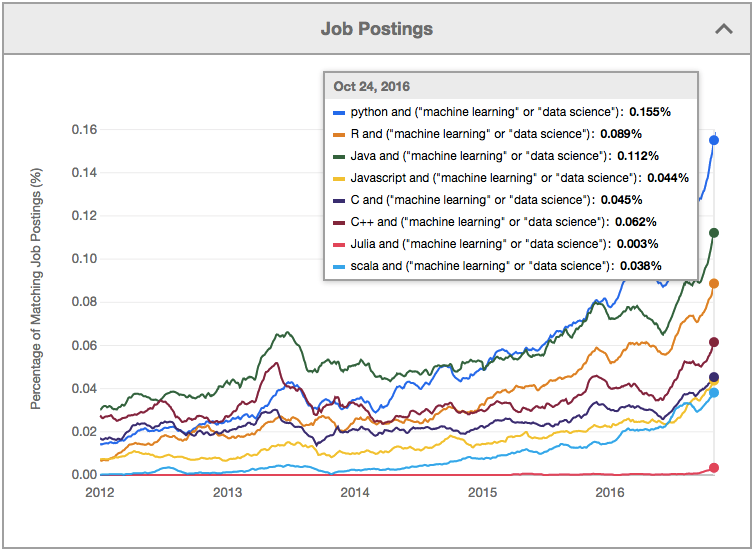
\includegraphics[keepaspectratio=true,scale=0.6]{__resources/top_lang.jpg}
		\caption{Graph of Machine Learning or Data Science Languages for 2016 by \cite{verma_2017}}
		\label{verma}
	\end{center}
\end{figure}

In light of the proclamations made above, it is clear that the preferred languages should be easy to learn, are backed by a large community, and is capable of complex mathematical operations. Also, it is desirable that the languages chosen for the proposed language is fast and efficient because of the complex computations that will occur during training.


\subsection{Machine Learning Framework}


\section{Data Preparation}

\subsection{Public Datasets}
\subsection{Creating a Dataset}



\section{Training}
\subsection{Training Locally}
\subsection{Cloud Training}

\section{Hosting/Deployment}

\section{Concluding Objective}
In conclusion, this section will outlines the objectives for the proposed project sequentially from the initial steps to the end product. The objectives are as follows:

\begin{itemize}
	\item Build a convolutional neural network for facial expression classification.
	\item Train the model on a large image data set.
	\item Save the train model and deploy it to a Python API.
	\item Develop a web application that is enabled to record a users facials expressions and send snapshots of the users face to the Python API in intervals.
	\item Use image preprocessing API on the webcam images for more accurate predictions.
	\item Use tone analyzer API for voice sentiment recognition.
	\item Weigh scores from the train model and tone analyzer accordingly and store them in a database
\end{itemize}

